% Created 2012-05-25 Fri 12:21
\documentclass[compress, 9pt]{beamer}
\usepackage[utf8]{inputenc}
\usepackage[T1]{fontenc}
\usepackage{fixltx2e}
\usepackage{graphicx}
\usepackage{longtable}
\usepackage{float}
\usepackage{wrapfig}
\usepackage{soul}
\usepackage{textcomp}
\usepackage{marvosym}
\usepackage{wasysym}
\usepackage{latexsym}
\usepackage{amssymb}
\tolerance=1000
\usetheme{default}
\usecolortheme[RGB={0,38,93}]{structure}
\usefonttheme{serif}
\useinnertheme{circles}
\useoutertheme[]{shadow}
\setbeamertemplate{navigation symbols}{}
\usepackage{natbib}
\usepackage{fleqn}
\usepackage{epsf}
\usepackage[dvips]{color}
\usepackage{bibentry}
\institute{Computer Science and Engineering \\ University of Michigan}
\providecommand{\alert}[1]{\textbf{#1}}

\title{Artificial Neural Networks \\~ Markov Decision Processes}
\author{Shiwali Mohan}
\date{\today}
\hypersetup{
  pdfkeywords={},
  pdfsubject={},
  pdfcreator={Emacs Org-mode version 7.8.09}}

\begin{document}

\maketitle

\begin{frame}
\frametitle{Outline}
\setcounter{tocdepth}{3}
\tableofcontents
\end{frame}


\title[Search \hspace{1em}\insertframenumber/
\inserttotalframenumber]{Full Title}


\section{Artificial Neural Networks}
\label{sec-1}
\begin{frame}
\frametitle{Perceptron Review}
\label{sec-1-1}

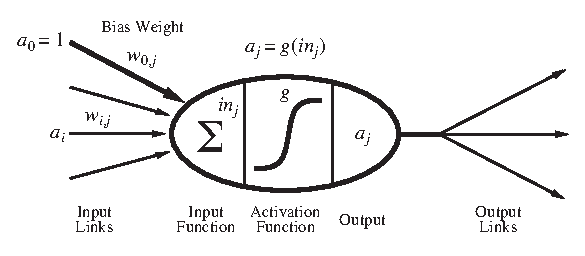
\includegraphics[width=10cm]{../images/neuron-unit.eps}
\end{frame}
\begin{frame}
\frametitle{Perceptron Design}
\label{sec-1-2}
\begin{itemize}

\item <1-> Implement $X \vee Y$ using a single perceptron unit. Assume bias input -1.
\label{sec-1-2-1}%
\end{itemize} % ends low level
\begin{columns}
\begin{column}{0.2\textwidth}
%% <2-> Image
\label{sec-1-2-2}

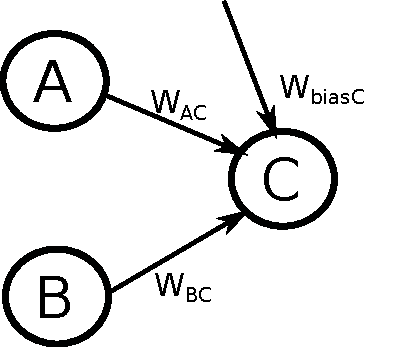
\includegraphics[width=4cm]{../images/nn.pdf}
\end{column}
\begin{column}{0.2\textwidth}
%% <2-> Table
\label{sec-1-2-3}


\begin{center}
\begin{tabular}{lr}
\hline
 W$_{\mathrm{AC}}$      &    1  \\
 W$_{\mathrm{BC}}$      &    1  \\
 W$_{\mathrm{bias,C}}$  &  0.5  \\
\hline
\end{tabular}
\end{center}
\end{column}
\end{columns}
\end{frame}
\begin{frame}
\frametitle{Perceptron Network Design}
\label{sec-1-3}
\begin{itemize}

\item <1-> Imlement $X \oplus Y$ using a preceptron network.
\label{sec-1-3-1}%
\end{itemize} % ends low level
\begin{columns}
\begin{column}{0.3\textwidth}
%% <2-> Image
\label{sec-1-3-2}

\includegraphics[width=6cm]{homework/nn2.pdf}
\end{column}
\begin{column}{0.5\textwidth}
%% <2-> Table
\label{sec-1-3-3}


\begin{center}
\begin{tabular}{lr}
\hline
 W$_{\mathrm{AC}}$      &    1  \\
 W$_{\mathrm{AD}}$      &   -1  \\
 W$_{\mathrm{BC}}$      &   -1  \\
 W$_{\mathrm{BD}}$      &    1  \\
 W$_{\mathrm{bias,C}}$  &  0.5  \\
 W$_{\mathrm{CE}}$      &    1  \\
 W$_{\mathrm{bias,D}}$  &  0.5  \\
 W$_{\mathrm{DE}}$      &    1  \\
 W$_{\mathrm{bias,E}}$  &  0.5  \\
\hline
\end{tabular}
\end{center}
\end{column}
\end{columns}
\end{frame}
\begin{frame}
\frametitle{Perceptron Network Design}
\label{sec-1-4}
\begin{itemize}

\item <1-> Suppose that after training for a long time, the weights of a 3 input (A, B, C) perceptron converge to the values Wa = 1, Wb = 0.5, Wc = 0.5, W0 = -0.75 (bias input is 1). Approximately what Boolean function has the perceptron learned? (Express in logical form as a function of the inputs A, B, and C. You can assume that the inputs take on values of either 0 (false) or 1 (true)). Use step function for activation.
\label{sec-1-4-1}%

\item <2->\\
\label{sec-1-4-2}%
\begin{center}
\begin{tabular}{rrrrrr}
\hline
 A  &  B  &  C  &  W0 (-0.75)  &  Sum(wx)  &  G(Sum(wx))  \\
\hline
 0  &  0  &  0  &           1  &    -0.75  &           0  \\
 0  &  0  &  1  &           1  &    -0.25  &           0  \\
 0  &  1  &  0  &           1  &    -0.25  &           0  \\
 0  &  1  &  1  &           1  &     0.25  &           1  \\
 1  &  0  &  0  &           1  &     0.25  &           1  \\
 1  &  0  &  1  &           1  &     0.75  &           1  \\
 1  &  1  &  0  &           1  &     0.75  &           1  \\
 1  &  1  &  1  &           1  &     1.25  &           1  \\
\hline
\end{tabular}
\end{center}



$A \vee B \wedge C$

\end{itemize} % ends low level
\end{frame}
\section{MDP and Learning}
\label{sec-2}
\begin{frame}
\frametitle{MDP review}
\label{sec-2-1}
\begin{itemize}

\item <1-> What kinds of problems can we reason about with MDPs?
\label{sec-2-1-1}%
\begin{itemize}

\item <2-> MDPs are used for making decisions about how to act in a world. The basic setup is that we have an agent who gets some information about the world, takes an action, gets a reward. The goal is to learn an action plan that will maximize reward.
\label{sec-2-1-1-1}%
\end{itemize} % ends low level

\item <3-> What is the Markov assumption?
\label{sec-2-1-2}%
\begin{itemize}

\item <4-> The future is independent of the past, given the present.
\label{sec-2-1-2-1}%
\end{itemize} % ends low level

\item <5-> How is an MDP defined?
\label{sec-2-1-3}%
\begin{itemize}

\item <6-> States, actions, transition models, rewards
\label{sec-2-1-3-1}%
\end{itemize} % ends low level

\item <7-> Algorithm for solving MDP.
\label{sec-2-1-4}%
\begin{itemize}

\item Value iteration.
\label{sec-2-1-4-1}%
\end{itemize} % ends low level
\end{itemize} % ends low level
\end{frame}
\begin{frame}
\frametitle{Value Iteration Example}
\label{sec-2-2}
\begin{columns}
\begin{column}{0.4\textwidth}
%% <2-> Image
\label{sec-2-2-1}

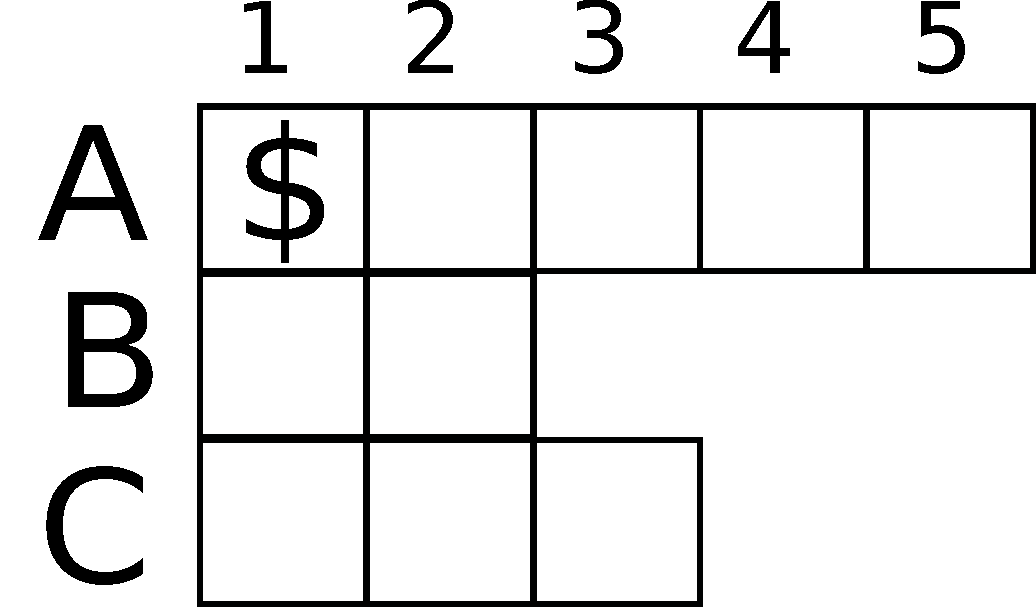
\includegraphics[width=5cm]{../images/domain.pdf}
\end{column}
\begin{column}{0.5\textwidth}
%% <2-> Data
\label{sec-2-2-2}


\begin{itemize}
\item \textbf{Actions}: forward, back, left, right, idle, pick-up
\item \textbf{Rewards}: pick-up treasure: 100, move: -5, idle: none
\item \textbf{Transition}: 0.8 move intended, 0.1 move to left, 0.1 move to right
\end{itemize}
\end{column}
\end{columns}
%% <3-> Questions
\label{sec-2-2-3}

\begin{itemize}
\item Formulate the problem as an MDP
\item Compute utilities and optimal policy in the first iteration.
\item In second iteration.
\item Sketch an optimal policy.
\end{itemize}
\end{frame}
\begin{frame}
\frametitle{Reinforcement Learning}
\label{sec-2-3}

\begin{itemize}
\item What if rewards were not known?
\item Review TD/Q learning.
\end{itemize}
\end{frame}

\end{document}
